\begin{frame}[label=sep_3v3_logloss]{Logloss: \var{Btrk1dR}, \var{Btrk2Pt}, \var{Btrk1Pt}}
\begin{columns}[T]
\column{0.49\textwidth}\centering\textbf{2018}\par\smallskip
\par\noindent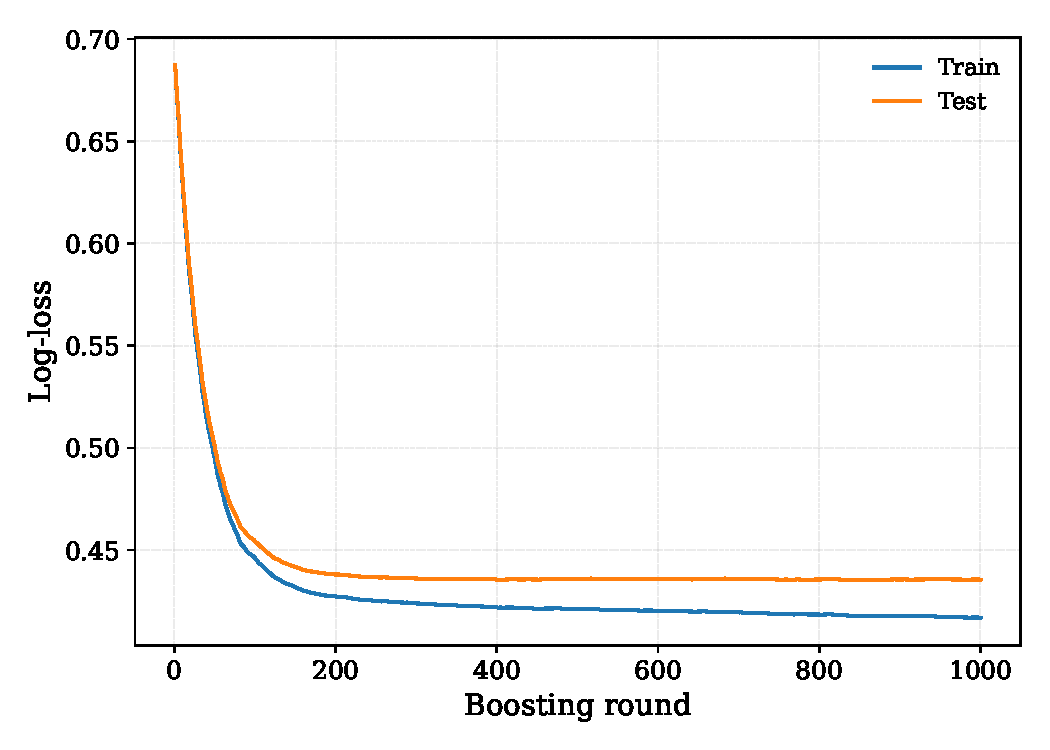
\includegraphics[width=\linewidth,height=0.62\textheight,keepaspectratio]{figures/20260930/X_pb18_v1_fid1_3v3_rw0_xgb_v1/logloss.pdf}
\column{0.49\textwidth}\centering\textbf{2023}\par\smallskip
\par\noindent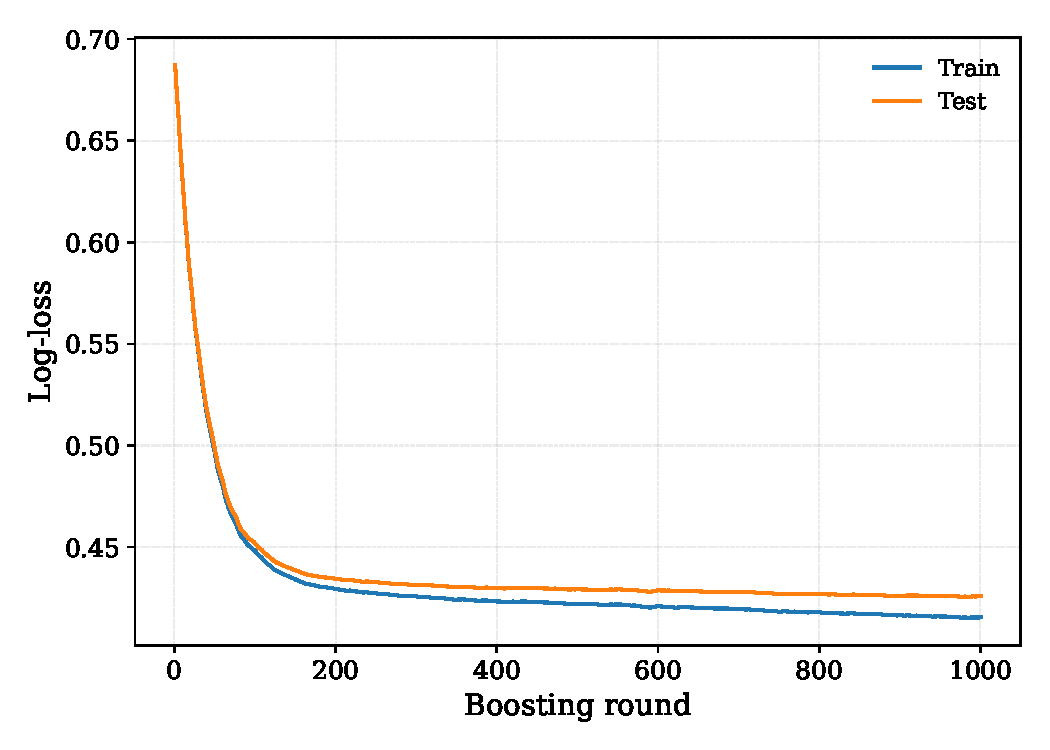
\includegraphics[width=\linewidth,height=0.62\textheight,keepaspectratio]{figures/20260930/X_pb23_v9_fid1_3v3_rw0_xgb_v1/logloss.pdf}
\end{columns}\small
1000 fixed training rounds; no early-stopping optimum.
\end{frame}

\begin{frame}[label=sep_3v3_roc]{ROC curve: \var{Btrk1dR}, \var{Btrk2Pt}, \var{Btrk1Pt}}
\begin{columns}[T]
\column{0.49\textwidth}\centering\textbf{2018}\par\smallskip
\par\noindent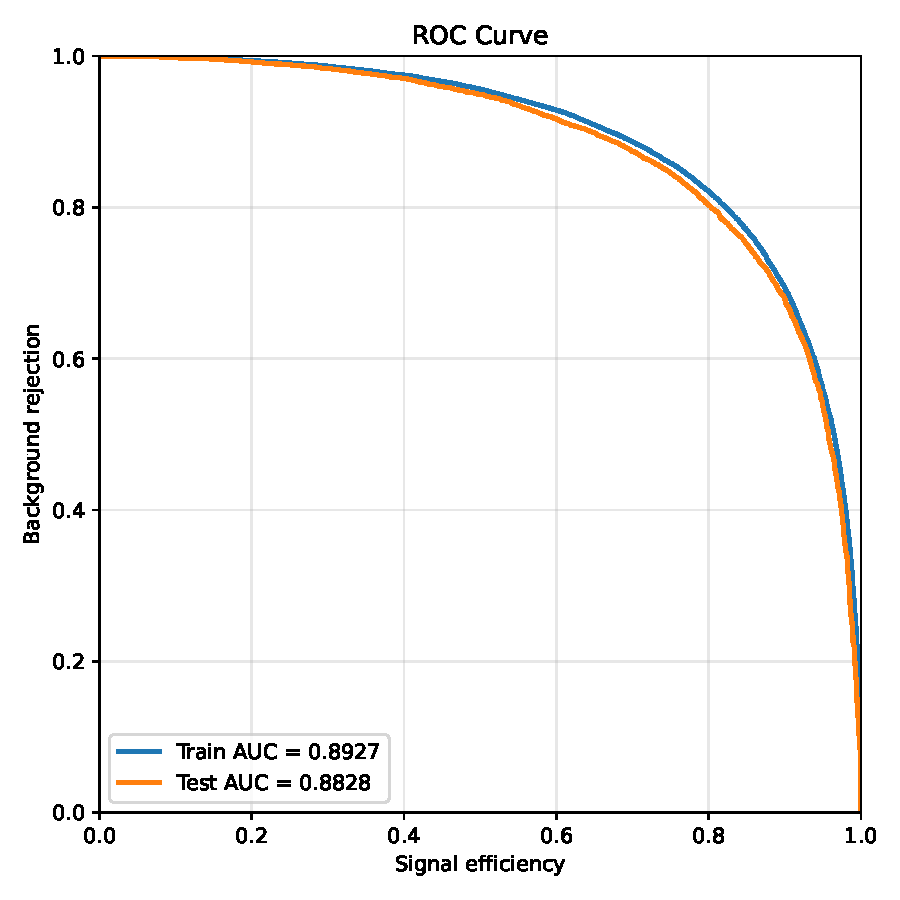
\includegraphics[width=\linewidth,height=0.62\textheight,keepaspectratio]{figures/20260930/X_pb18_v1_fid1_3v3_rw0_xgb_v1/roc.pdf}
\column{0.49\textwidth}\centering\textbf{2023}\par\smallskip
\par\noindent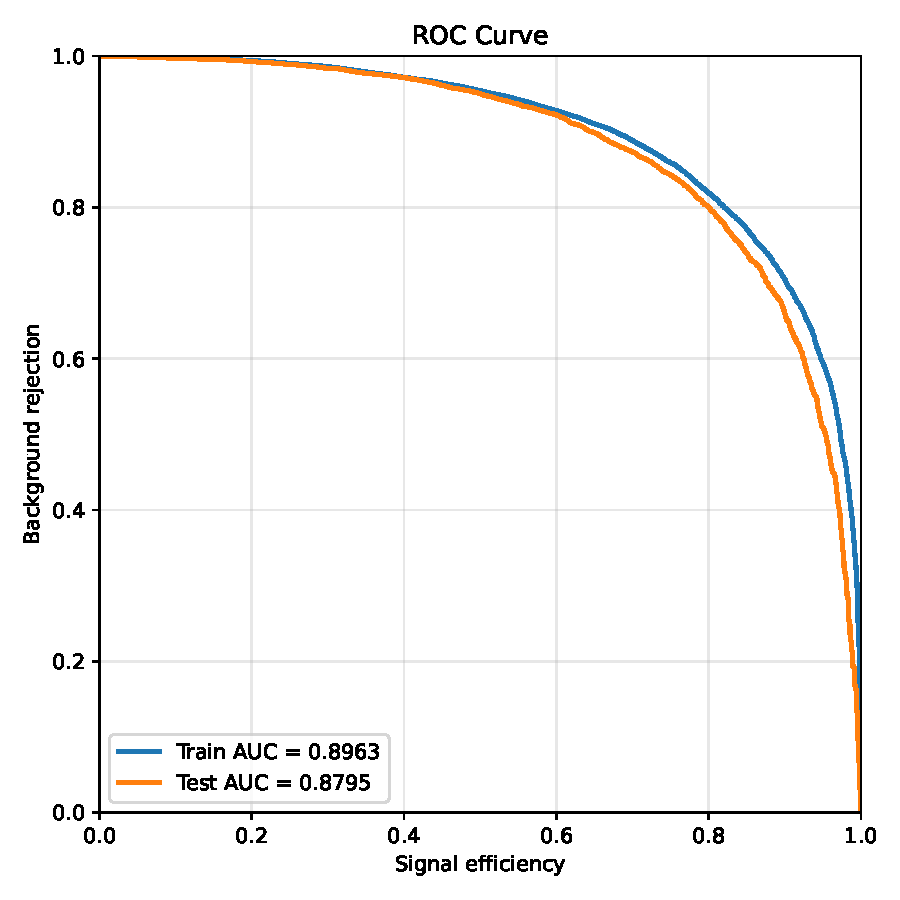
\includegraphics[width=\linewidth,height=0.62\textheight,keepaspectratio]{figures/20260930/X_pb23_v9_fid1_3v3_rw0_xgb_v1/roc.pdf}
\end{columns}\small
Signal: physical MC weights; background: unit weights. Train/test and pooled curves retain their original definitions.
\end{frame}

\begin{frame}[label=sep_3v3_shap_bar]{Cumulative SHAP: \var{Btrk1dR}, \var{Btrk2Pt}, \var{Btrk1Pt}}
\begin{columns}[T]
\column{0.49\textwidth}\centering\textbf{2018}\par\smallskip
\par\noindent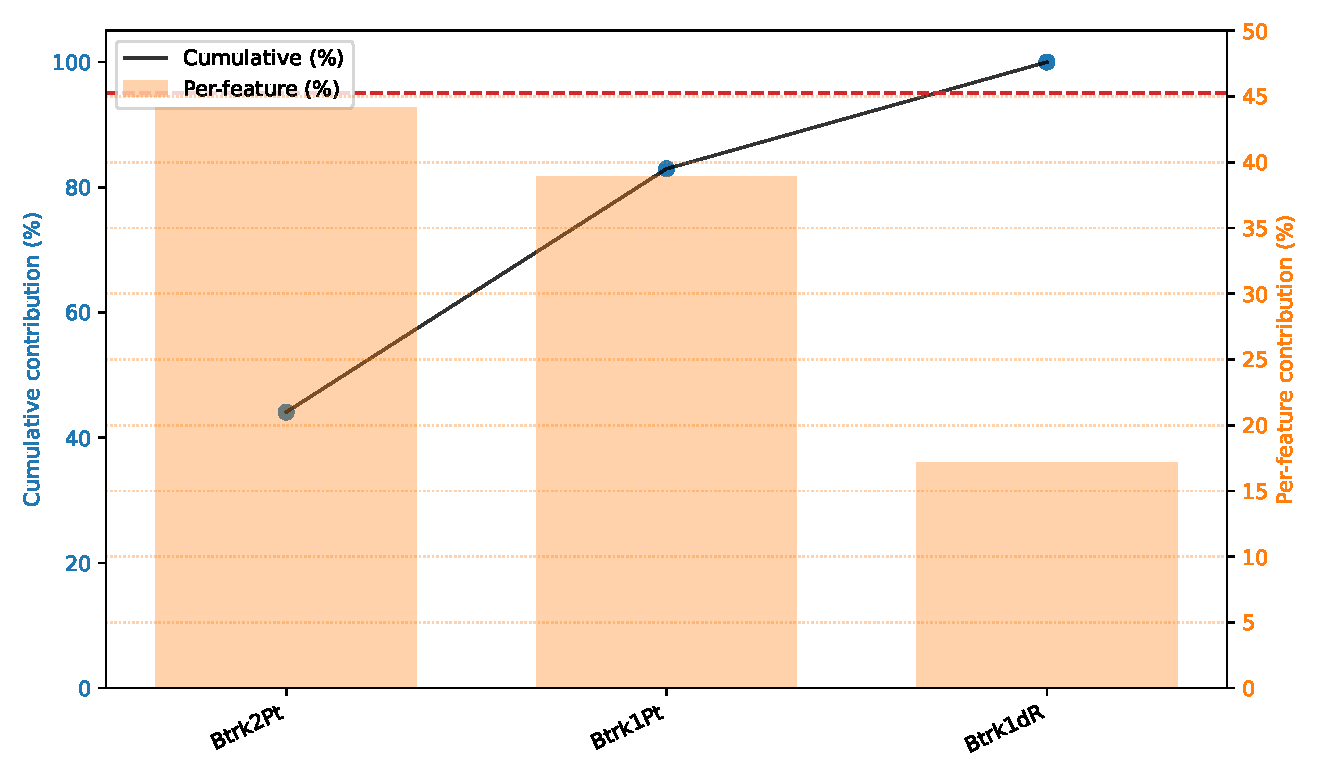
\includegraphics[width=\linewidth,height=0.62\textheight,keepaspectratio]{figures/20260930/X_pb18_v1_fid1_3v3_rw0_xgb_v1/shap_cumulative.pdf}
\column{0.49\textwidth}\centering\textbf{2023}\par\smallskip
\par\noindent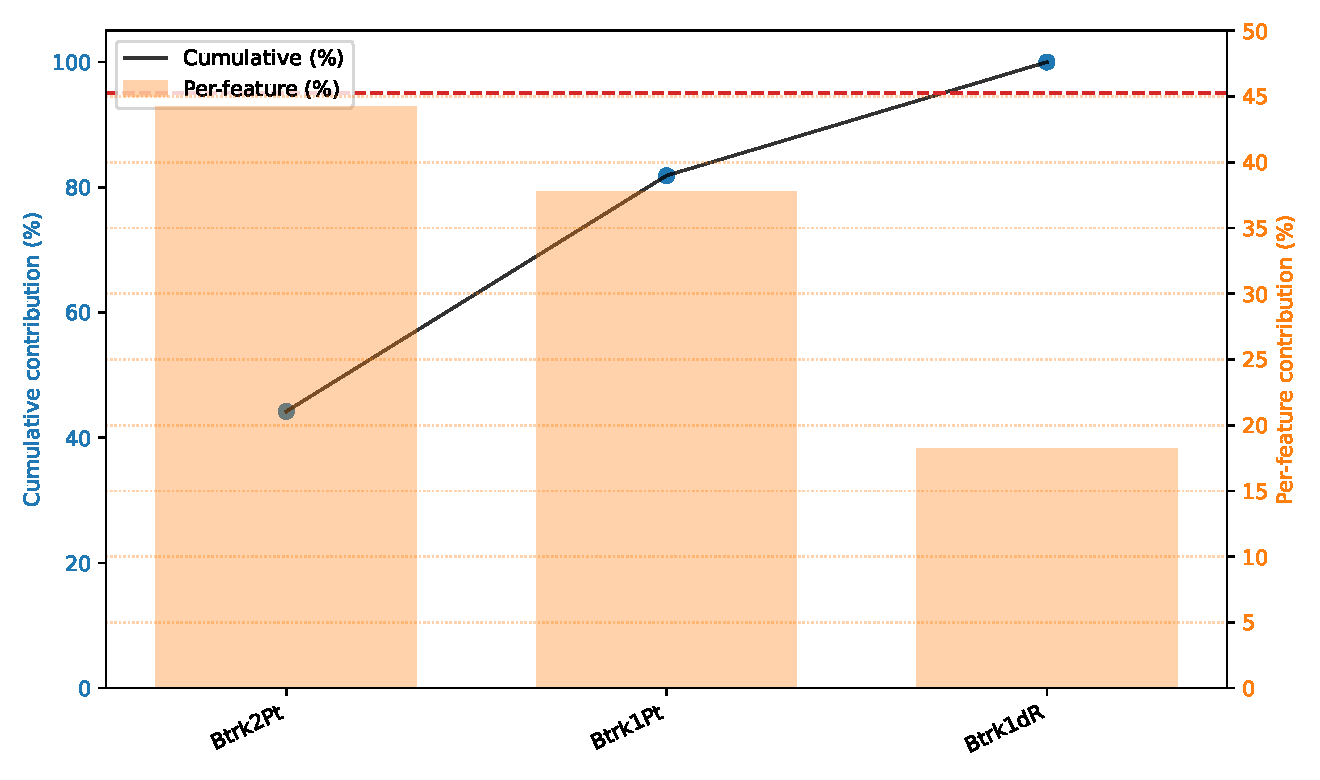
\includegraphics[width=\linewidth,height=0.62\textheight,keepaspectratio]{figures/20260930/X_pb23_v9_fid1_3v3_rw0_xgb_v1/shap_cumulative.pdf}
\end{columns}\small
Cumulative weighted mean $|\mathrm{SHAP}|$ on a mixed signal/background sample.
\end{frame}

\begin{frame}[label=sep_3v7_logloss]{Logloss: \var{BtrkLeadPt}, \var{BtrkSubPt}, \var{BtrkMaxdR}}
\begin{columns}[T]
\column{0.49\textwidth}\centering\textbf{2018}\par\smallskip
\par\noindent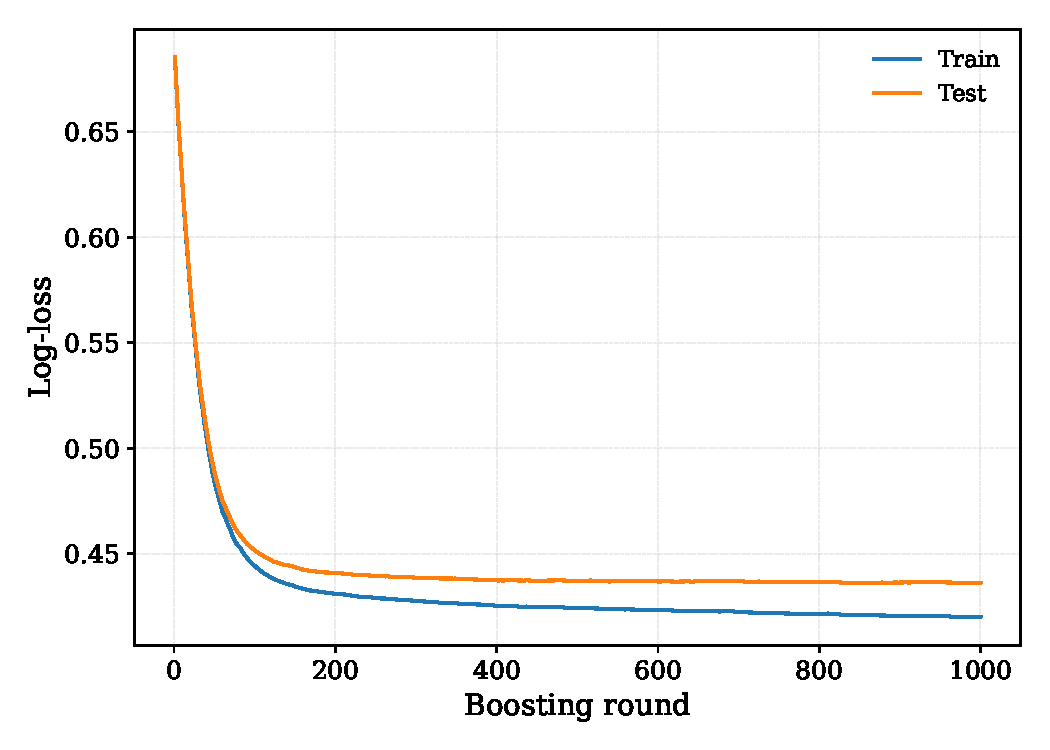
\includegraphics[width=\linewidth,height=0.62\textheight,keepaspectratio]{figures/20260930/X_pb18_v1_fid1_3v7_rw0_xgb_v1/logloss.pdf}
\column{0.49\textwidth}\centering\textbf{2023}\par\smallskip
\par\noindent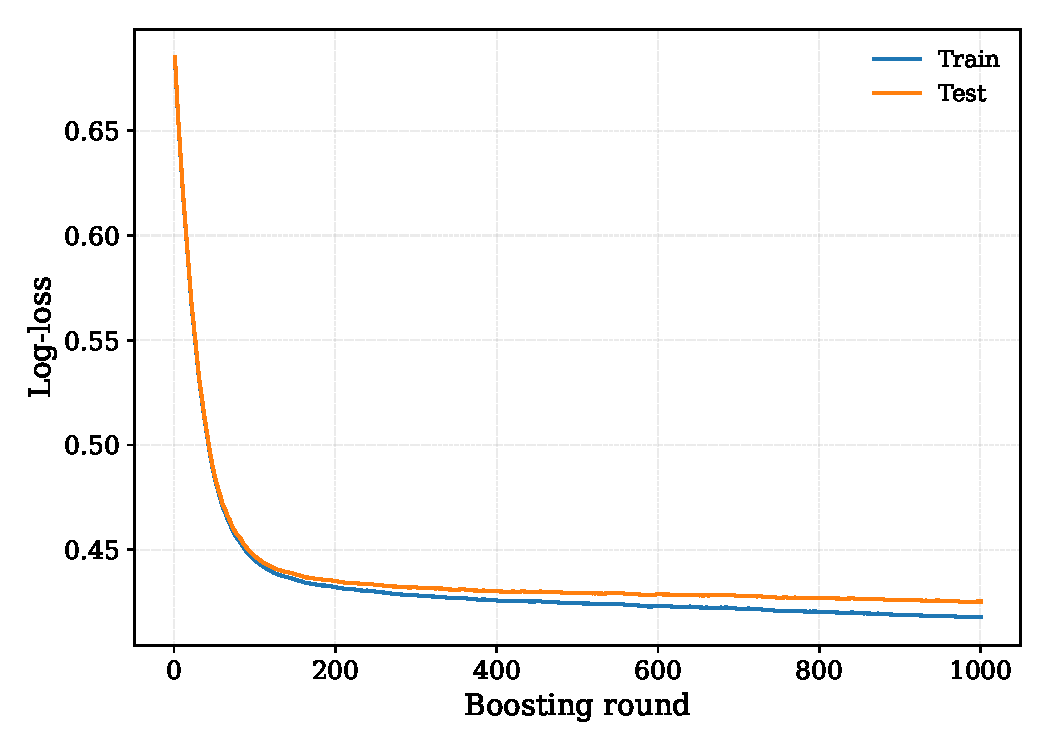
\includegraphics[width=\linewidth,height=0.62\textheight,keepaspectratio]{figures/20260930/X_pb23_v9_fid1_3v7_rw0_xgb_v1/logloss.pdf}
\end{columns}\small
1000 fixed training rounds; no early-stopping optimum.
\end{frame}

\begin{frame}[label=sep_3v7_roc]{ROC curve: \var{BtrkLeadPt}, \var{BtrkSubPt}, \var{BtrkMaxdR}}
\begin{columns}[T]
\column{0.49\textwidth}\centering\textbf{2018}\par\smallskip
\par\noindent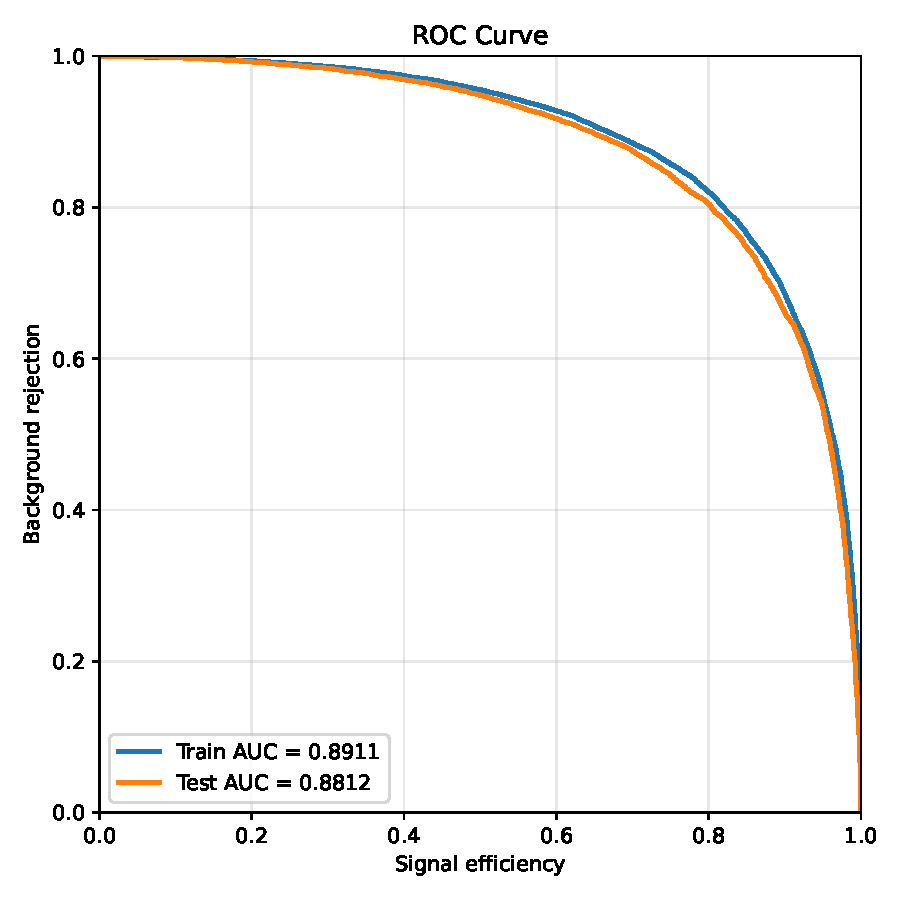
\includegraphics[width=\linewidth,height=0.62\textheight,keepaspectratio]{figures/20260930/X_pb18_v1_fid1_3v7_rw0_xgb_v1/roc.pdf}
\column{0.49\textwidth}\centering\textbf{2023}\par\smallskip
\par\noindent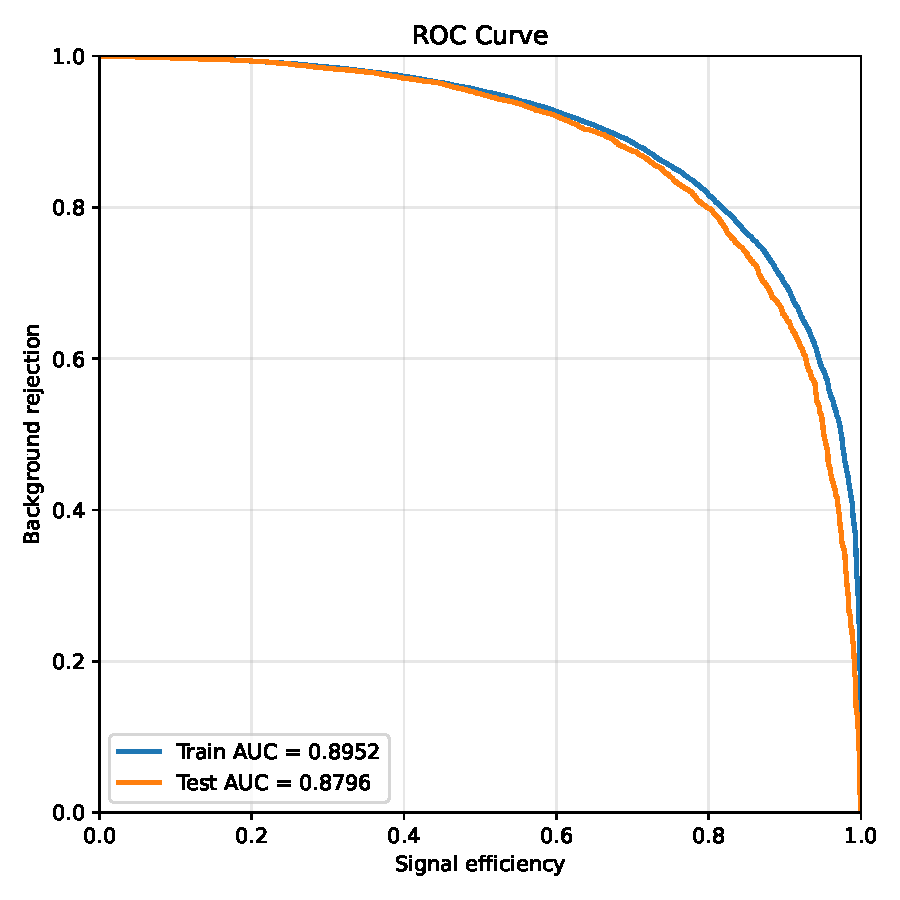
\includegraphics[width=\linewidth,height=0.62\textheight,keepaspectratio]{figures/20260930/X_pb23_v9_fid1_3v7_rw0_xgb_v1/roc.pdf}
\end{columns}\small
Signal: physical MC weights; background: unit weights. Train/test and pooled curves retain their original definitions.
\end{frame}

\begin{frame}[label=sep_3v7_shap_bar]{Cumulative SHAP: \var{BtrkLeadPt}, \var{BtrkSubPt}, \var{BtrkMaxdR}}
\begin{columns}[T]
\column{0.49\textwidth}\centering\textbf{2018}\par\smallskip
\par\noindent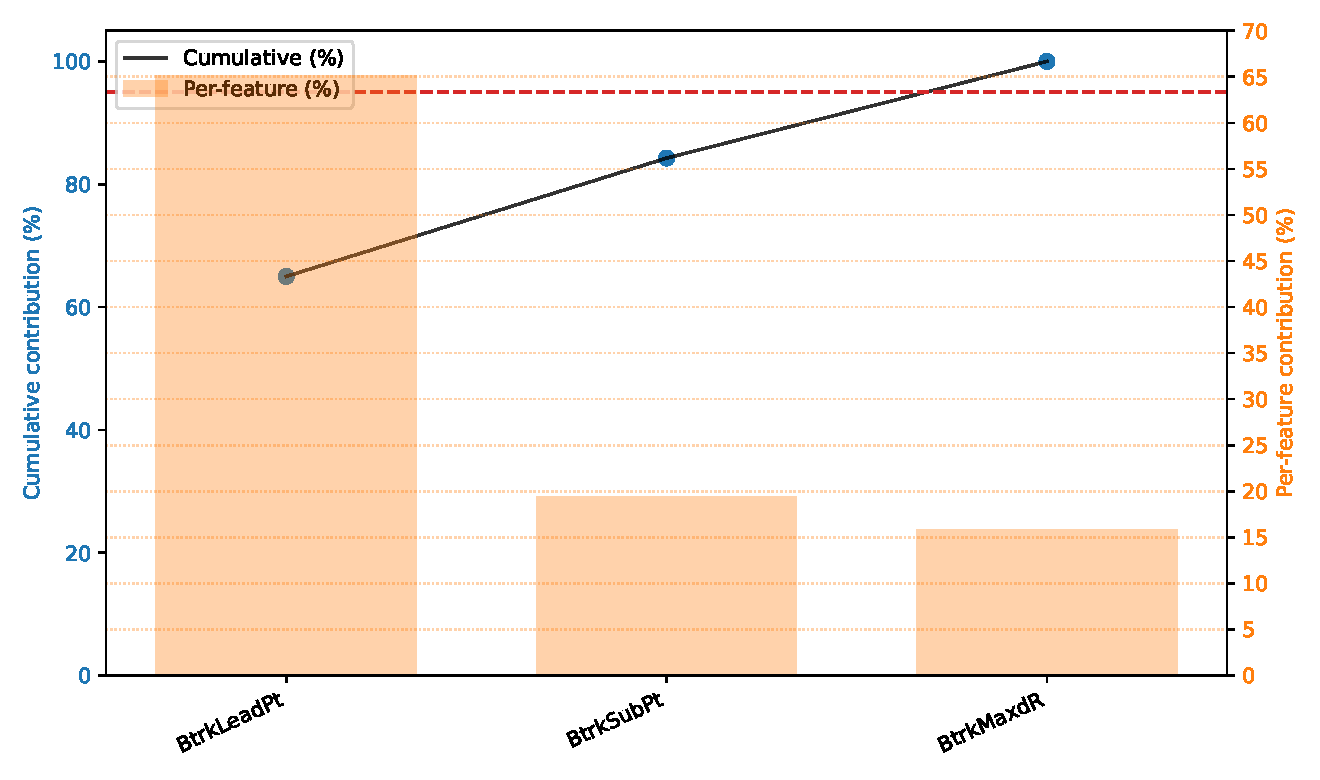
\includegraphics[width=\linewidth,height=0.62\textheight,keepaspectratio]{figures/20260930/X_pb18_v1_fid1_3v7_rw0_xgb_v1/shap_cumulative.pdf}
\column{0.49\textwidth}\centering\textbf{2023}\par\smallskip
\par\noindent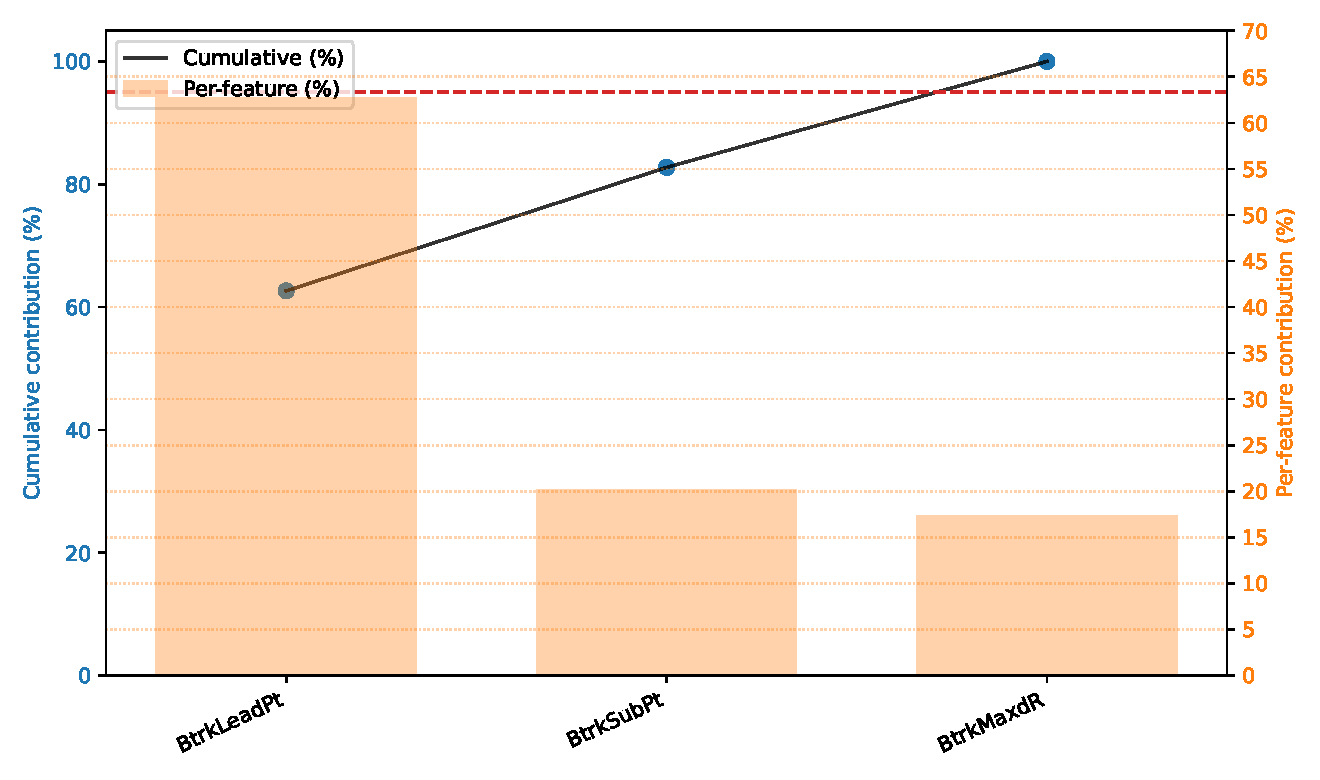
\includegraphics[width=\linewidth,height=0.62\textheight,keepaspectratio]{figures/20260930/X_pb23_v9_fid1_3v7_rw0_xgb_v1/shap_cumulative.pdf}
\end{columns}\small
Cumulative weighted mean $|\mathrm{SHAP}|$ on a mixed signal/background sample.
\end{frame}

\begin{frame}[label=sep_back_9v1]{9v1: combined 2018 + 2023 fit}
\noindent{\small 9v1: \var{Bmu1pt}, \var{Bmu1eta}, \var{Bmu2pt}, \var{Bmu2eta}, \var{Btrk2Pt}, \var{BtrkPtimb}, \var{Btrk1dR}, \var{Bujeta}, \var{Btktketa}.\par}\smallskip
\begin{columns}[T]
\column{0.49\textwidth}\centering\small\textbf{2018}\quad score $>0.88$\
\par\noindent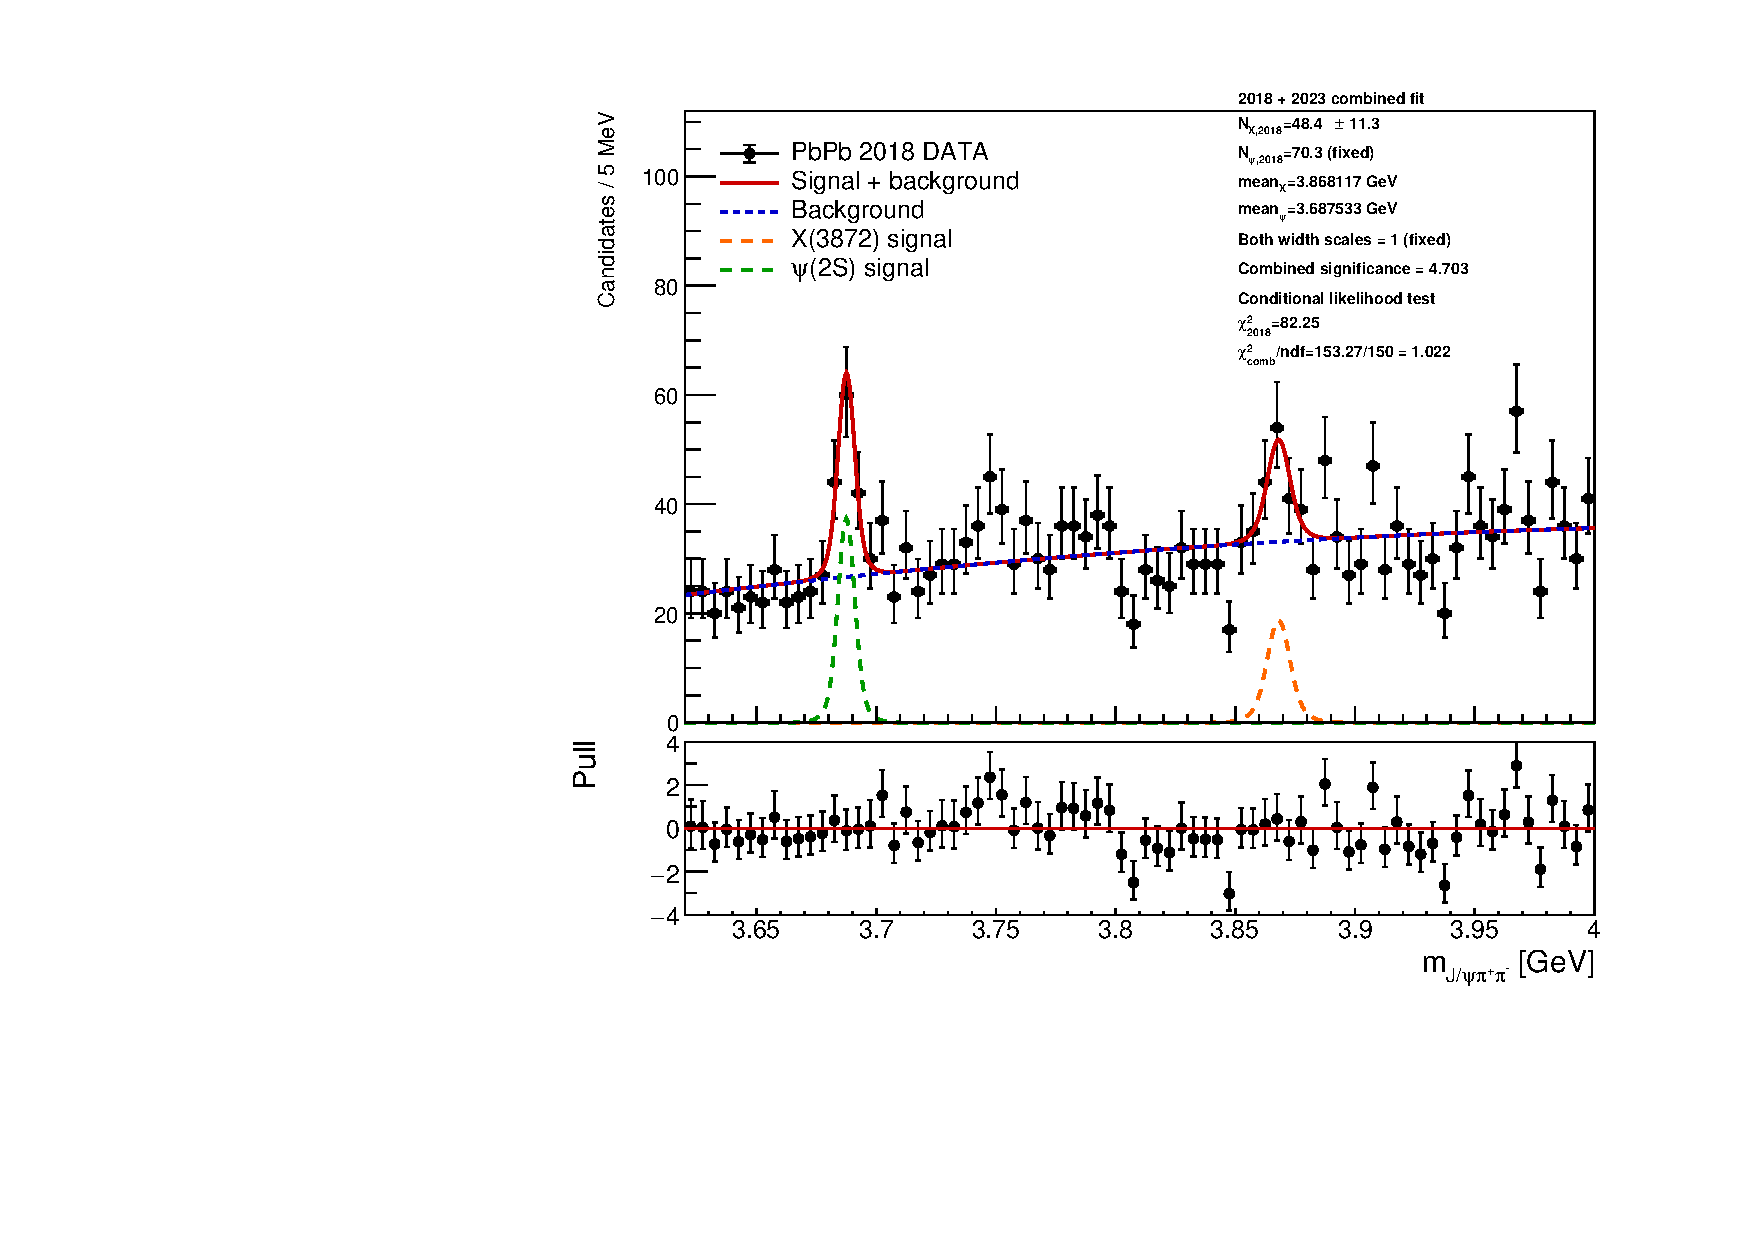
\includegraphics[width=\linewidth,height=0.50\textheight,keepaspectratio]{figures/20260930/9v1/pb18_conditional_fit.pdf}
\column{0.49\textwidth}\centering\small\textbf{2023}\quad score $>0.85$\
\par\noindent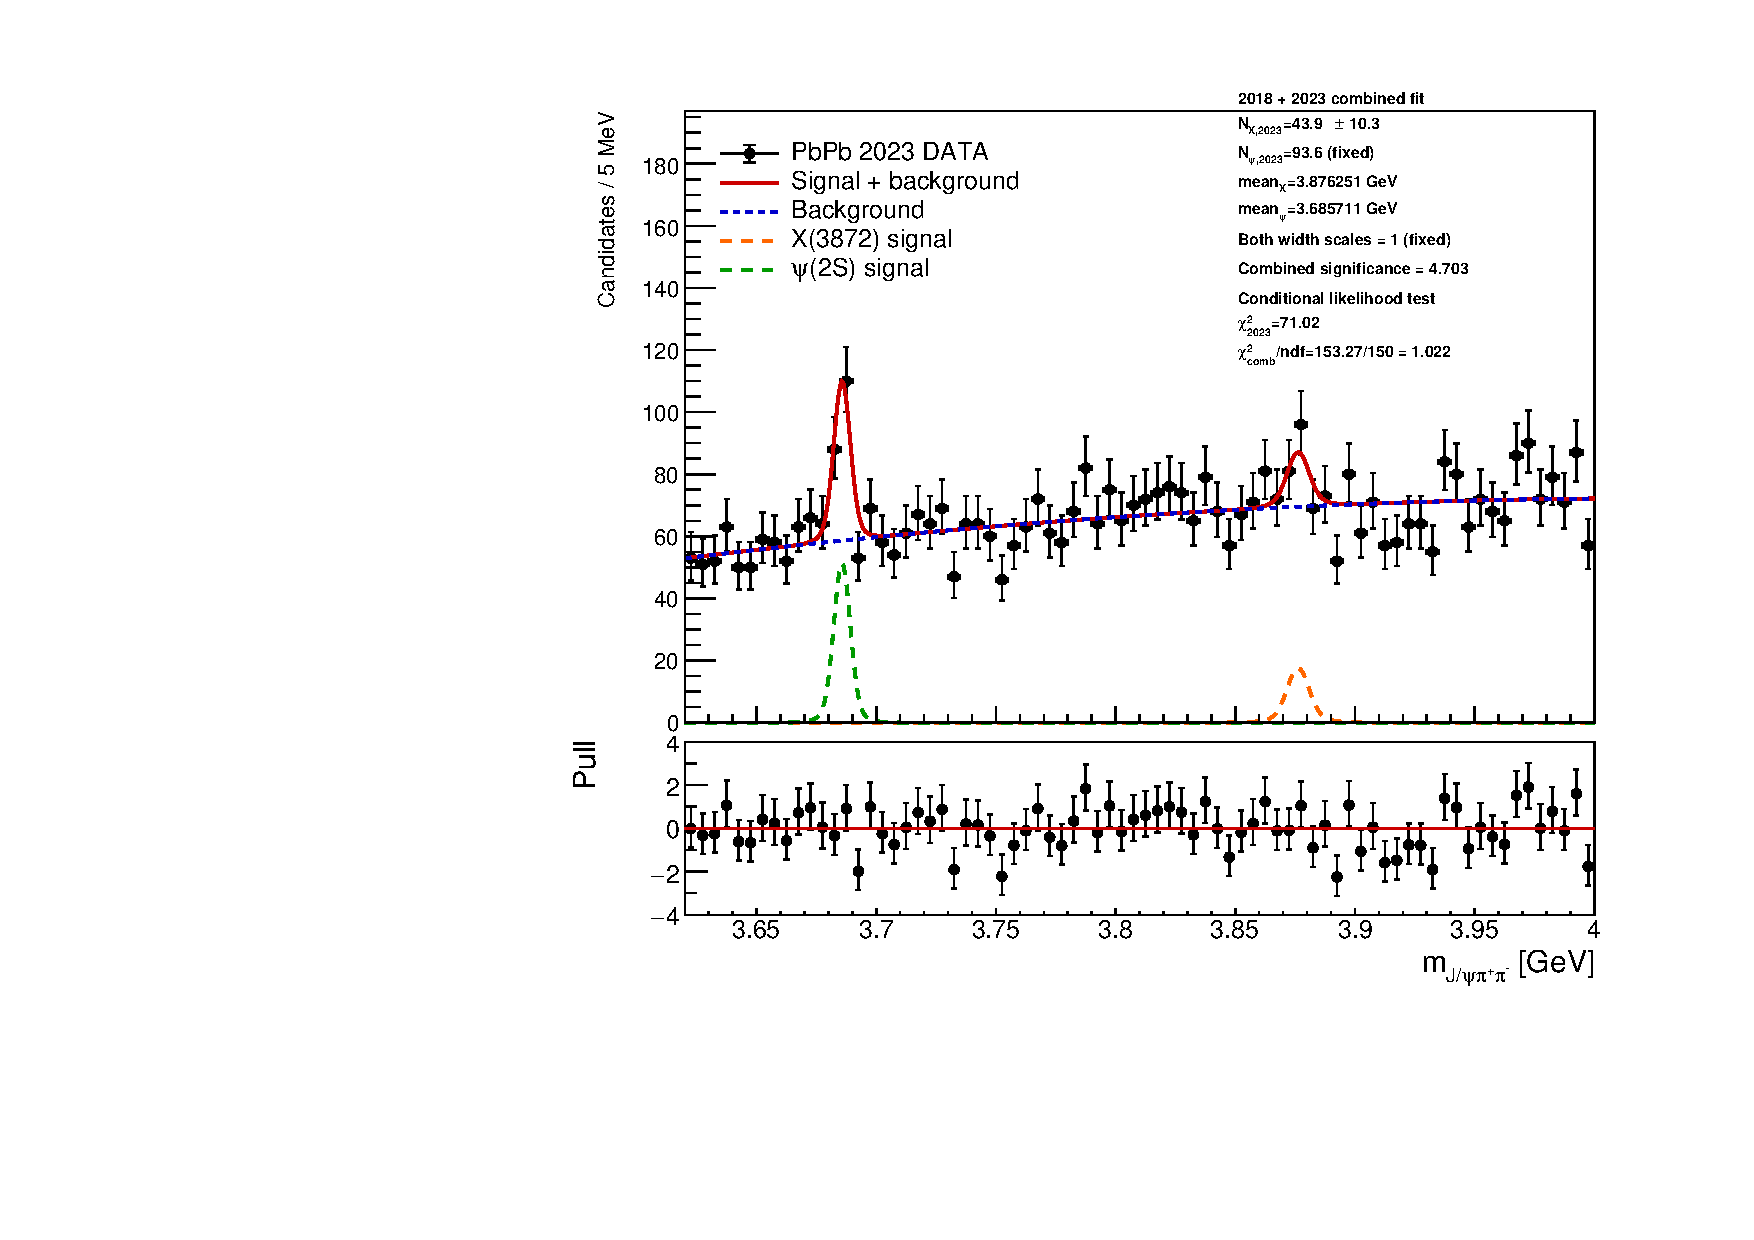
\includegraphics[width=\linewidth,height=0.50\textheight,keepaspectratio]{figures/20260930/9v1/pb23_conditional_fit.pdf}
\end{columns}\small
\textbf{Combined:} $N_X=92.27\pm21.52$; significance $=4.703\sigma$.\par
\textbf{Independent-year reference:} 2018: $3.903\sigma$; 2023: $2.587\sigma$.\par
\textbf{Combined:} $\chi^2/\mathrm{ndf}=1.022$.\par
\caution{MC double-Gaussian widths fixed; 2nd-order Chebyshev background.}

\end{frame}

\begin{frame}[label=sep_back_5v1]{5v1: combined 2018 + 2023 fit}
\noindent{\small 5v1: \var{Bmu1pt}, \var{Bmu2pt}, \var{Btrk2Pt}, \var{BtrkPtimb}, \var{Btrk1dR}.\par}\smallskip
\begin{columns}[T]
\column{0.49\textwidth}\centering\small\textbf{2018}\quad score $>0.89$\
\par\noindent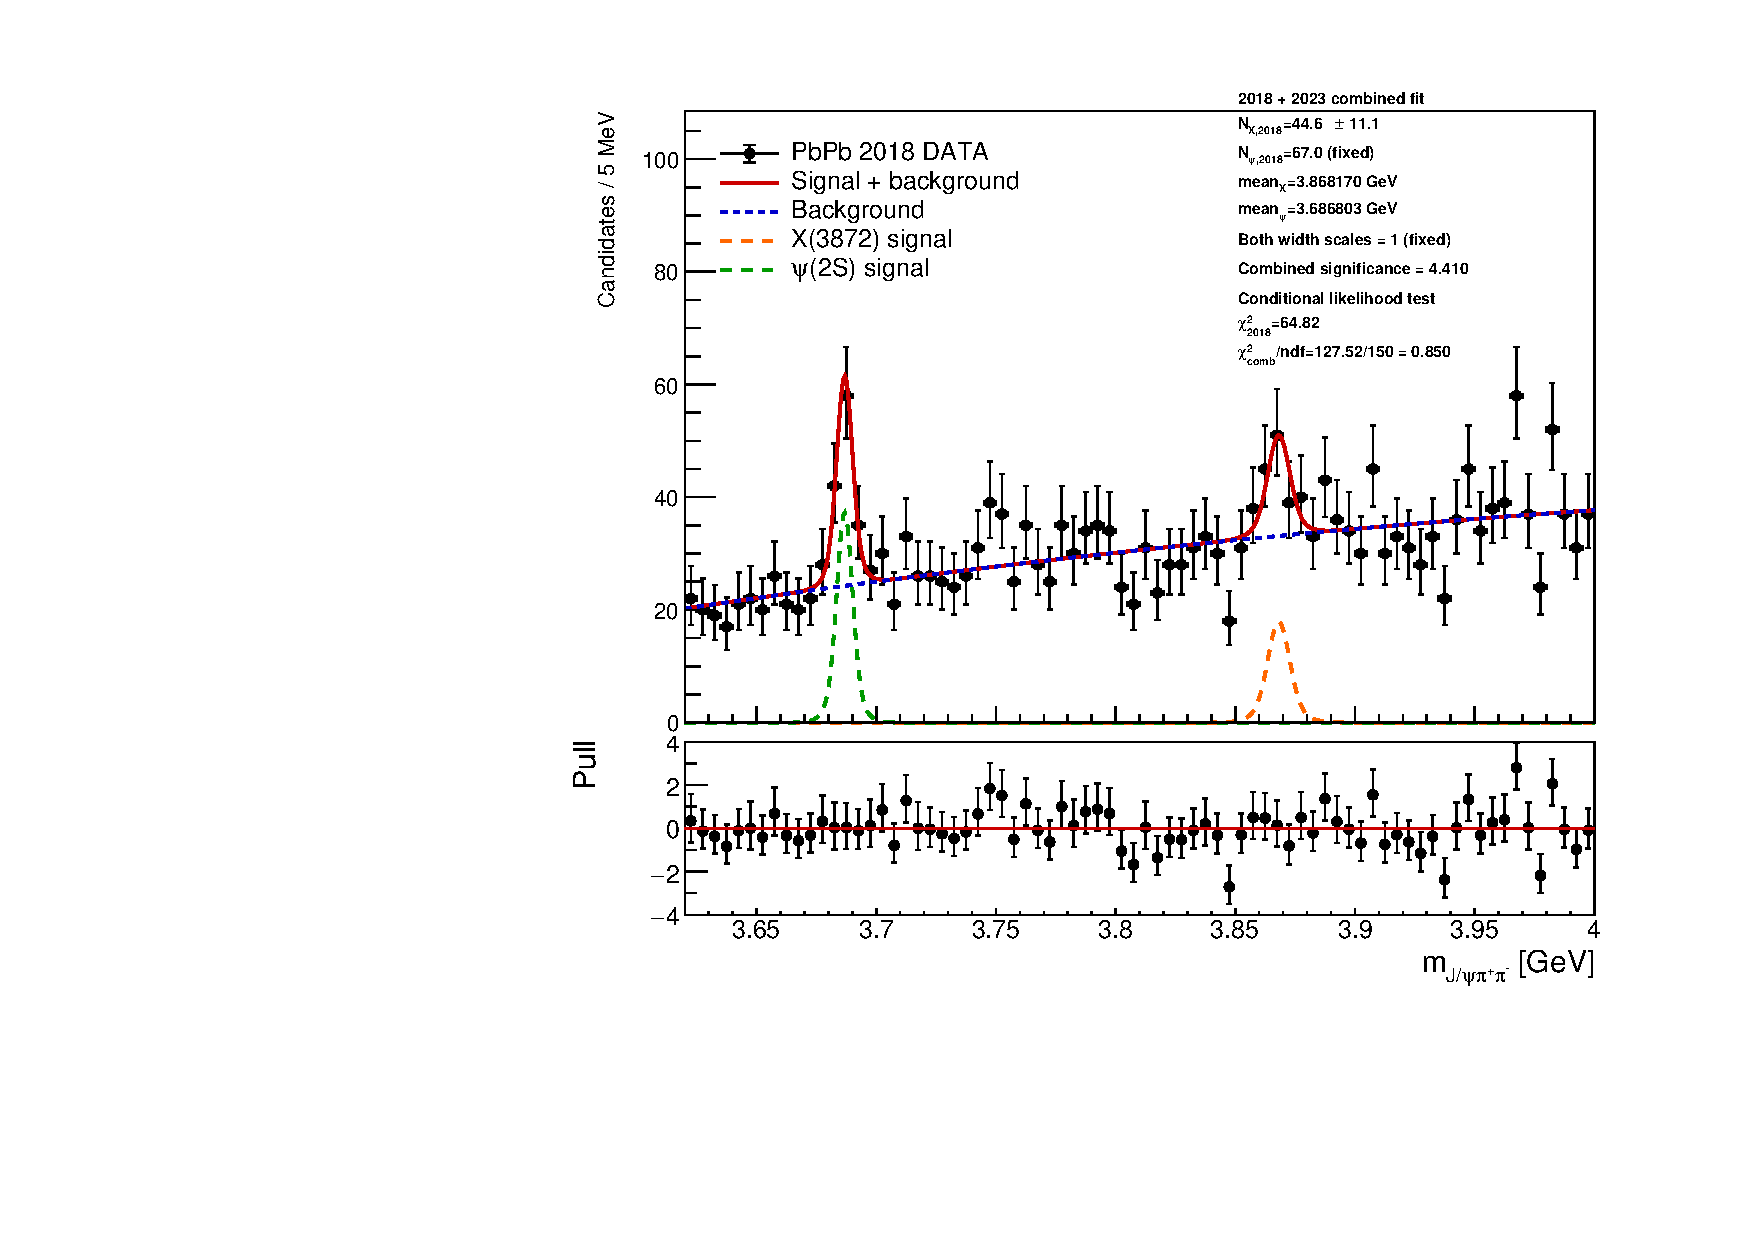
\includegraphics[width=\linewidth,height=0.50\textheight,keepaspectratio]{figures/20260930/5v1/pb18_conditional_fit.pdf}
\column{0.49\textwidth}\centering\small\textbf{2023}\quad score $>0.85$\
\par\noindent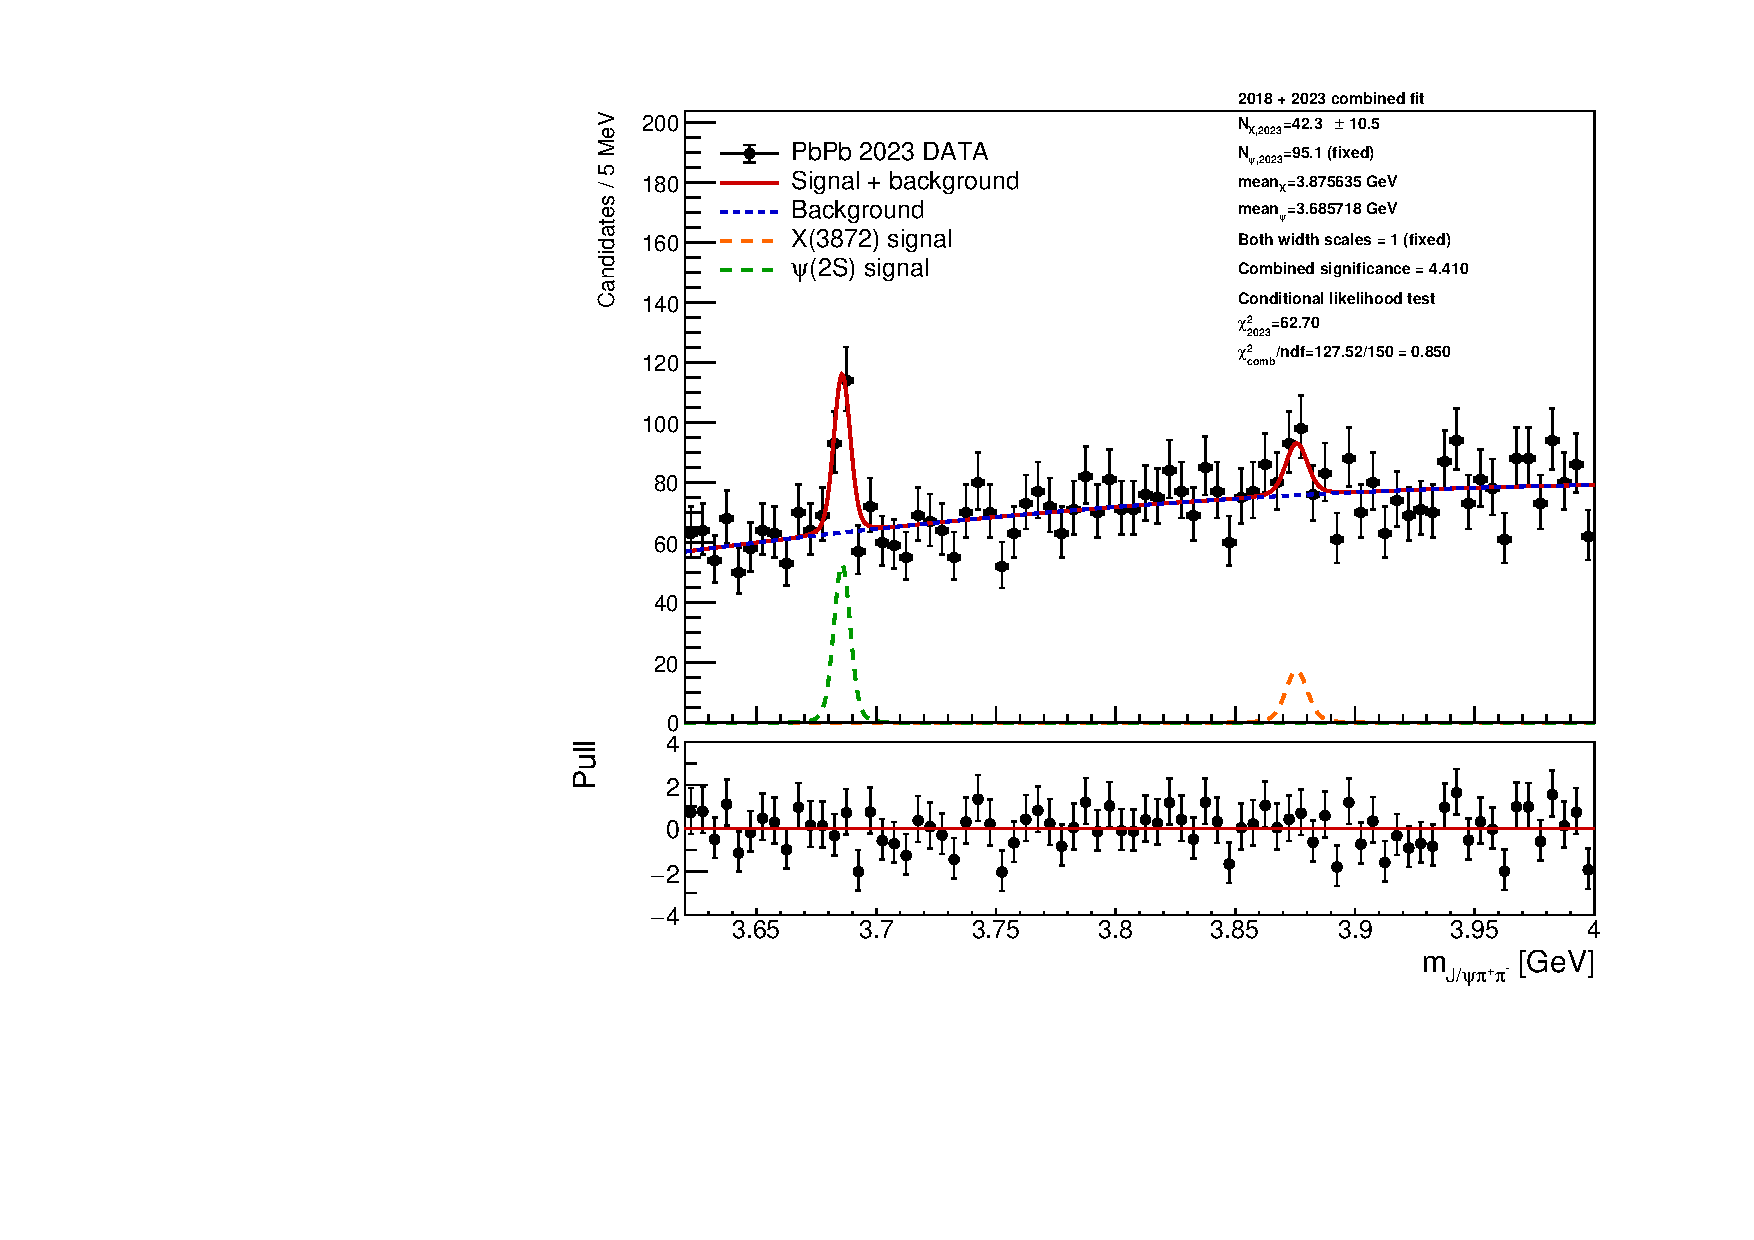
\includegraphics[width=\linewidth,height=0.50\textheight,keepaspectratio]{figures/20260930/5v1/pb23_conditional_fit.pdf}
\end{columns}\small
\textbf{Combined:} $N_X=86.96\pm21.56$; significance $=4.410\sigma$.\par
\textbf{Independent-year reference:} 2018: $3.671\sigma$; 2023: $2.397\sigma$.\par
\textbf{Combined:} $\chi^2/\mathrm{ndf}=0.850$.\par
\caution{MC double-Gaussian widths fixed; 2nd-order Chebyshev background.}

\end{frame}

\begin{frame}[label=sep_back_3v5]{Combined fit: \var{Btrk1dR}, \var{Btrk2Pt}, \var{BtrkPtimb}}
\begin{columns}[T]
\column{0.49\textwidth}\centering\small\textbf{2018}\quad score $>0.83$\
\par\noindent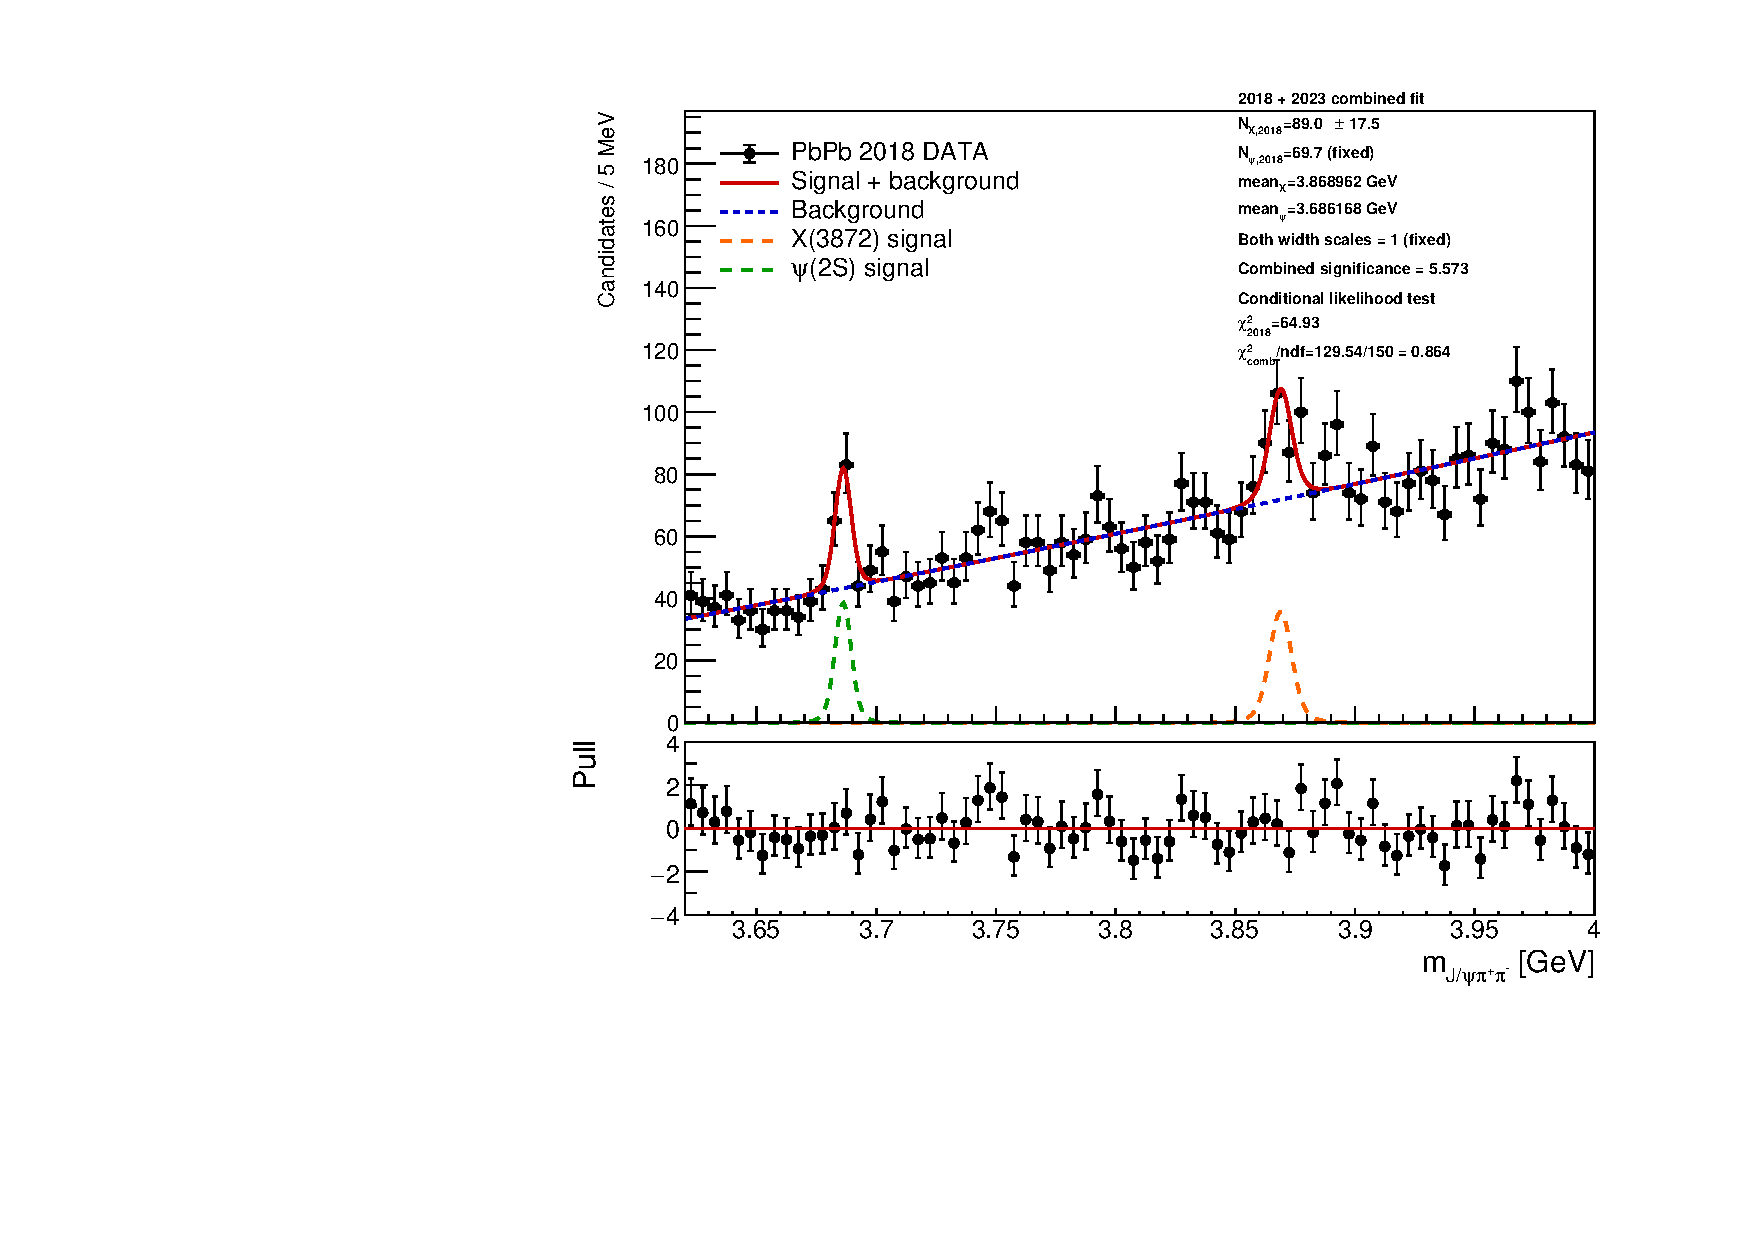
\includegraphics[width=\linewidth,height=0.58\textheight,keepaspectratio]{figures/20260930/3v5/pb18_conditional_fit.pdf}
\column{0.49\textwidth}\centering\small\textbf{2023}\quad score $>0.80$\
\par\noindent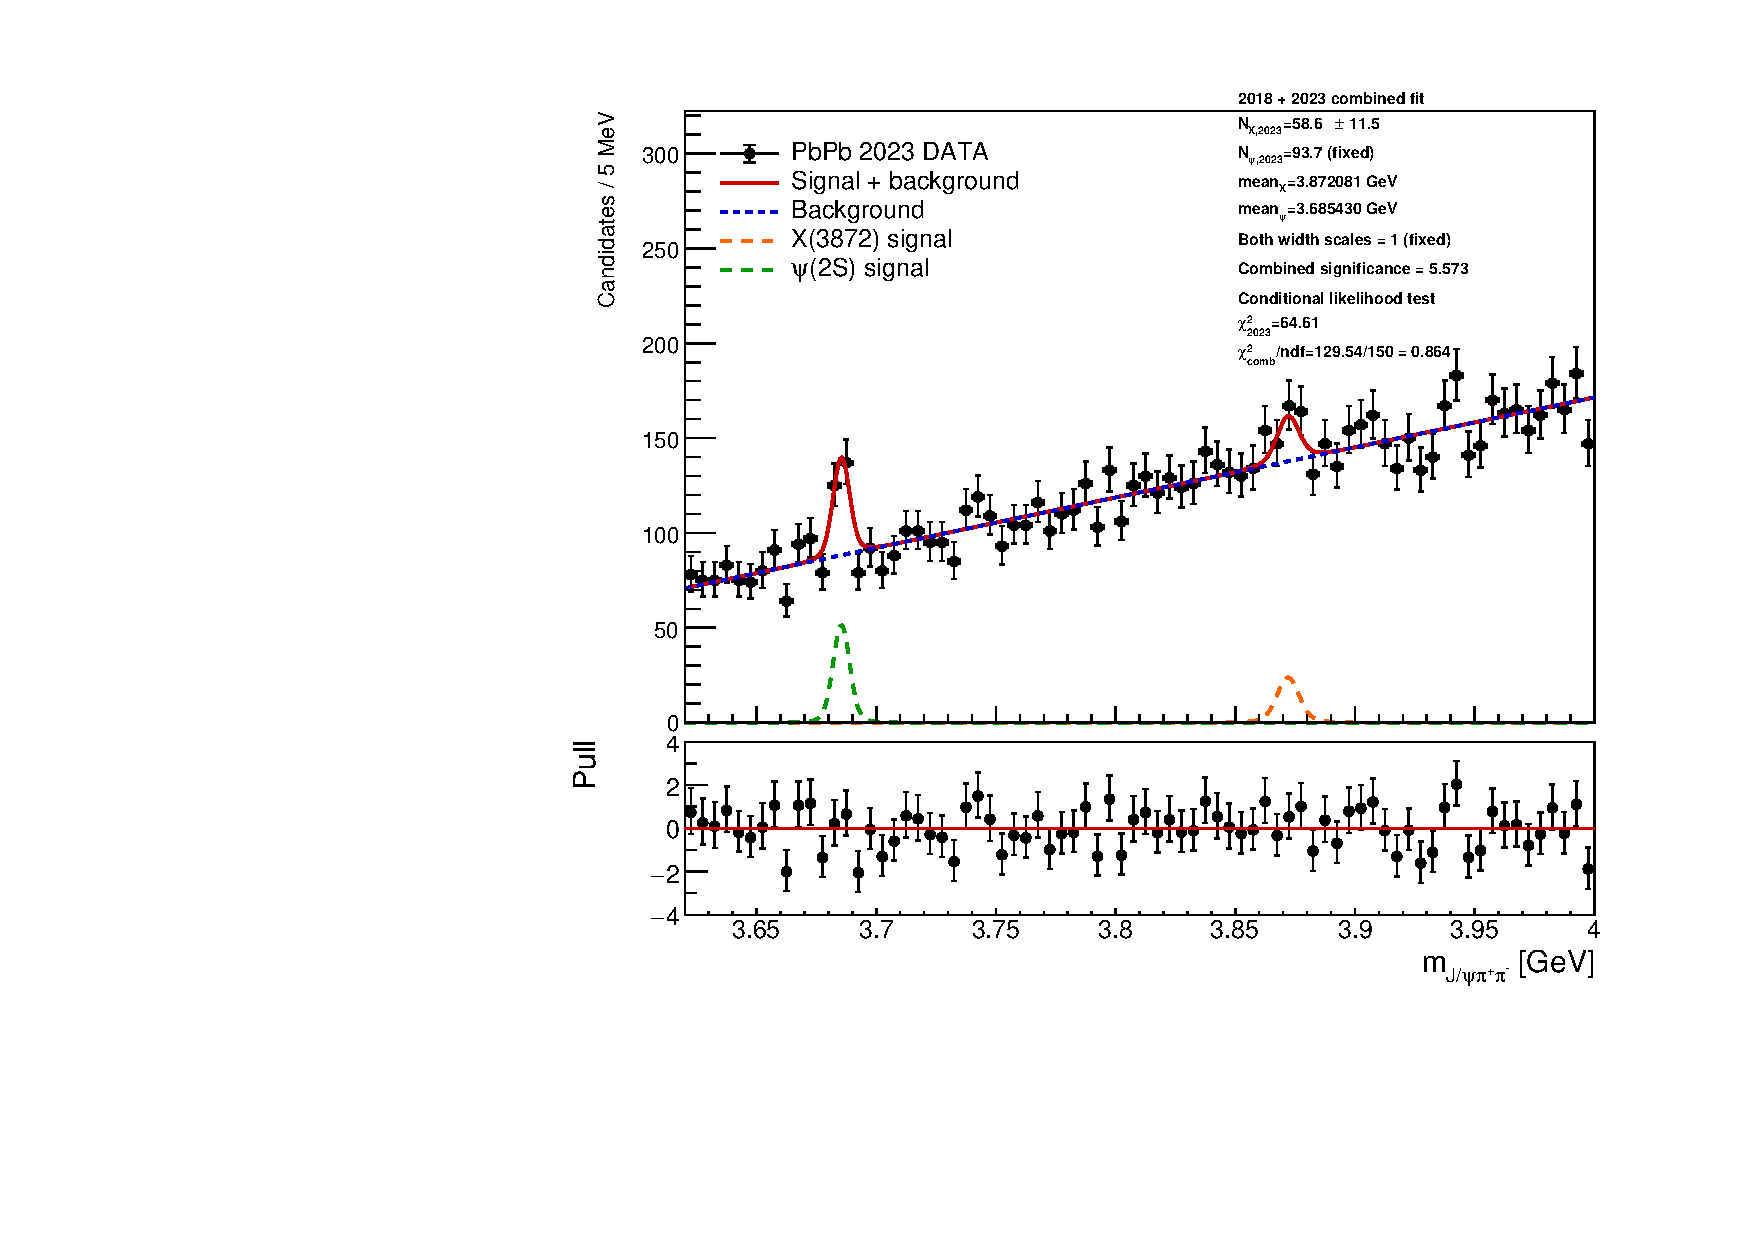
\includegraphics[width=\linewidth,height=0.58\textheight,keepaspectratio]{figures/20260930/3v5/pb23_conditional_fit.pdf}
\end{columns}\small
\textbf{Combined:} $N_X=147.69\pm28.94$; significance $=5.573\sigma$.\par
\textbf{Independent-year reference:} 2018: $4.949\sigma$; 2023: $2.466\sigma$.\par
\textbf{Combined:} $\chi^2/\mathrm{ndf}=0.864$.\par
\caution{MC double-Gaussian widths fixed; 2nd-order Chebyshev background.}

\end{frame}

\begin{frame}[label=sep_back_3v12]{Combined fit: \var{BtrkLeadPt}, \var{BtrkPtimb}, \var{BtrkMaxdR}}
\begin{columns}[T]
\column{0.49\textwidth}\centering\small\textbf{2018}\quad score $>0.85$\
\par\noindent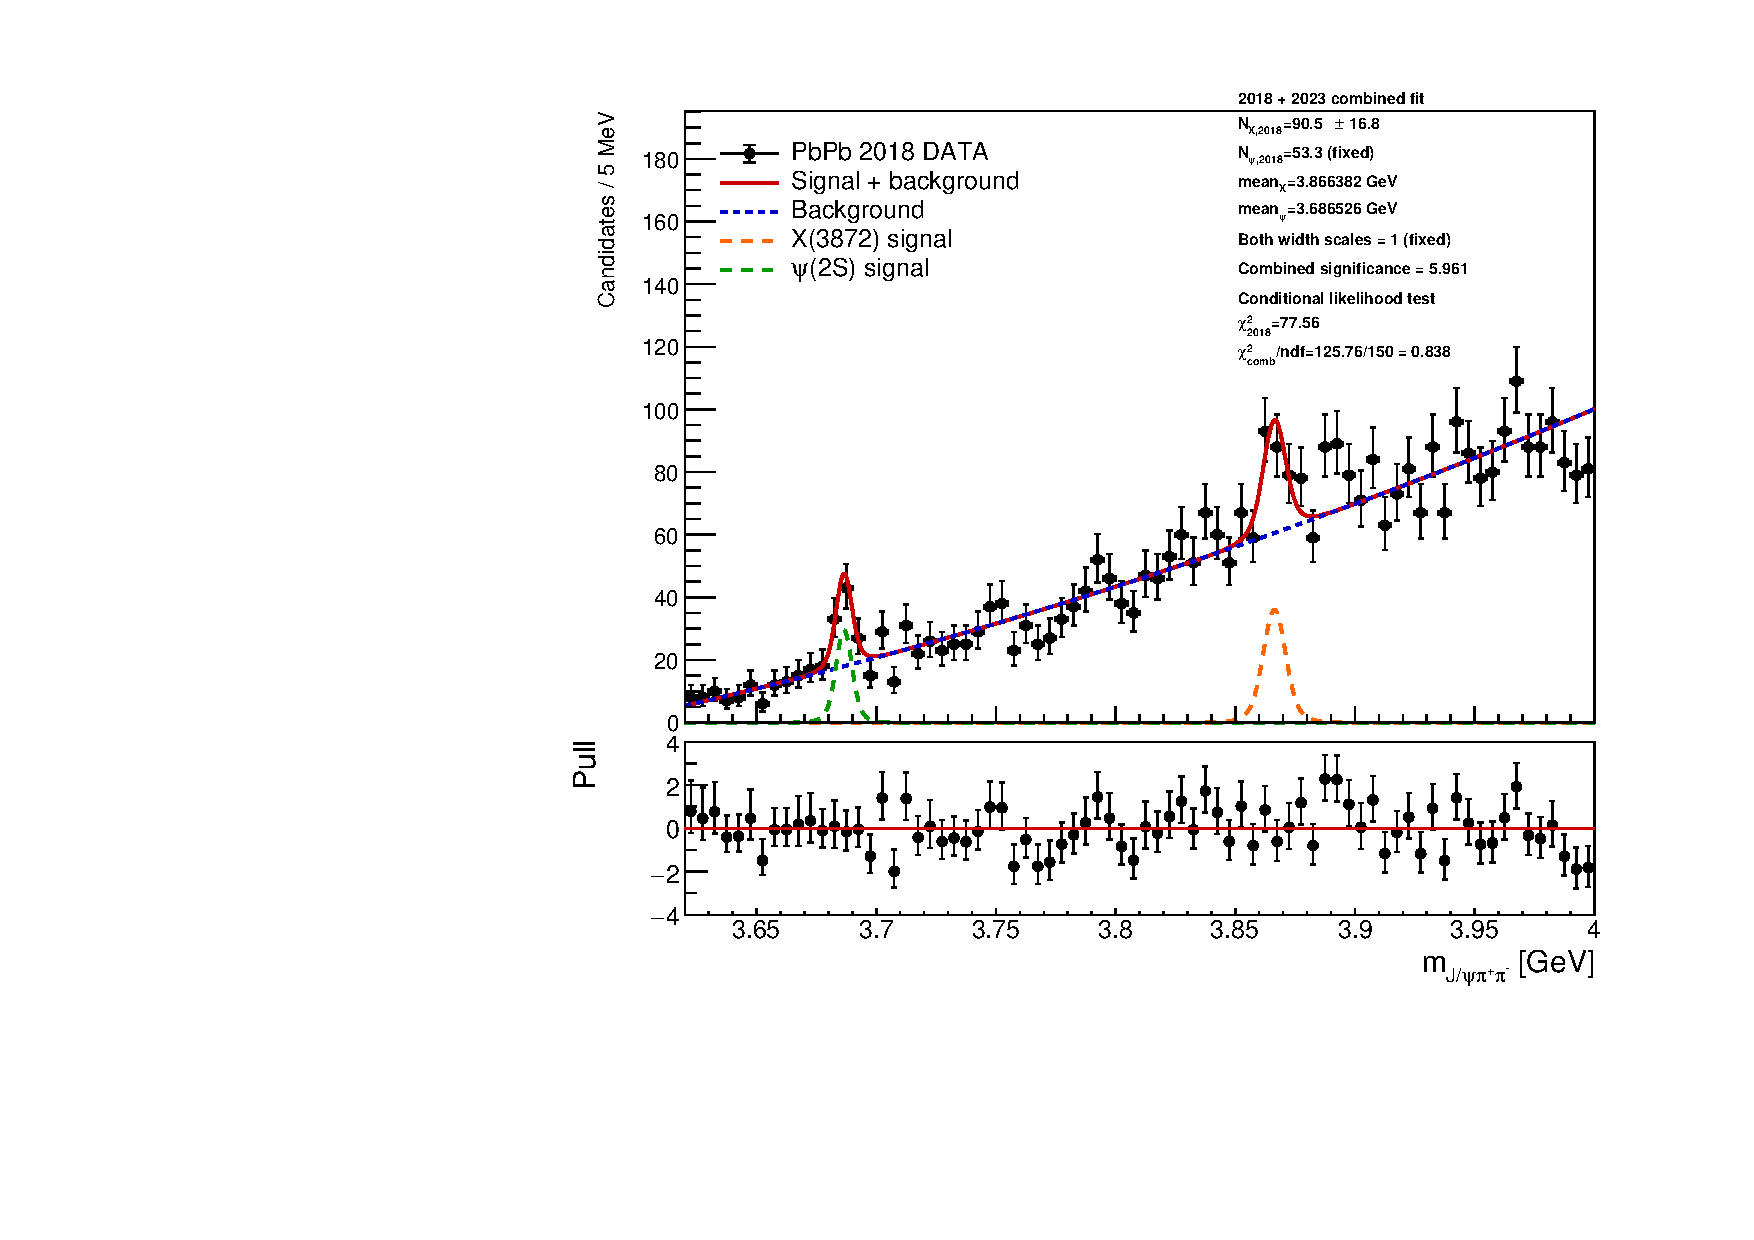
\includegraphics[width=\linewidth,height=0.58\textheight,keepaspectratio]{figures/20260930/3v12/pb18_conditional_fit.pdf}
\column{0.49\textwidth}\centering\small\textbf{2023}\quad score $>0.88$\
\par\noindent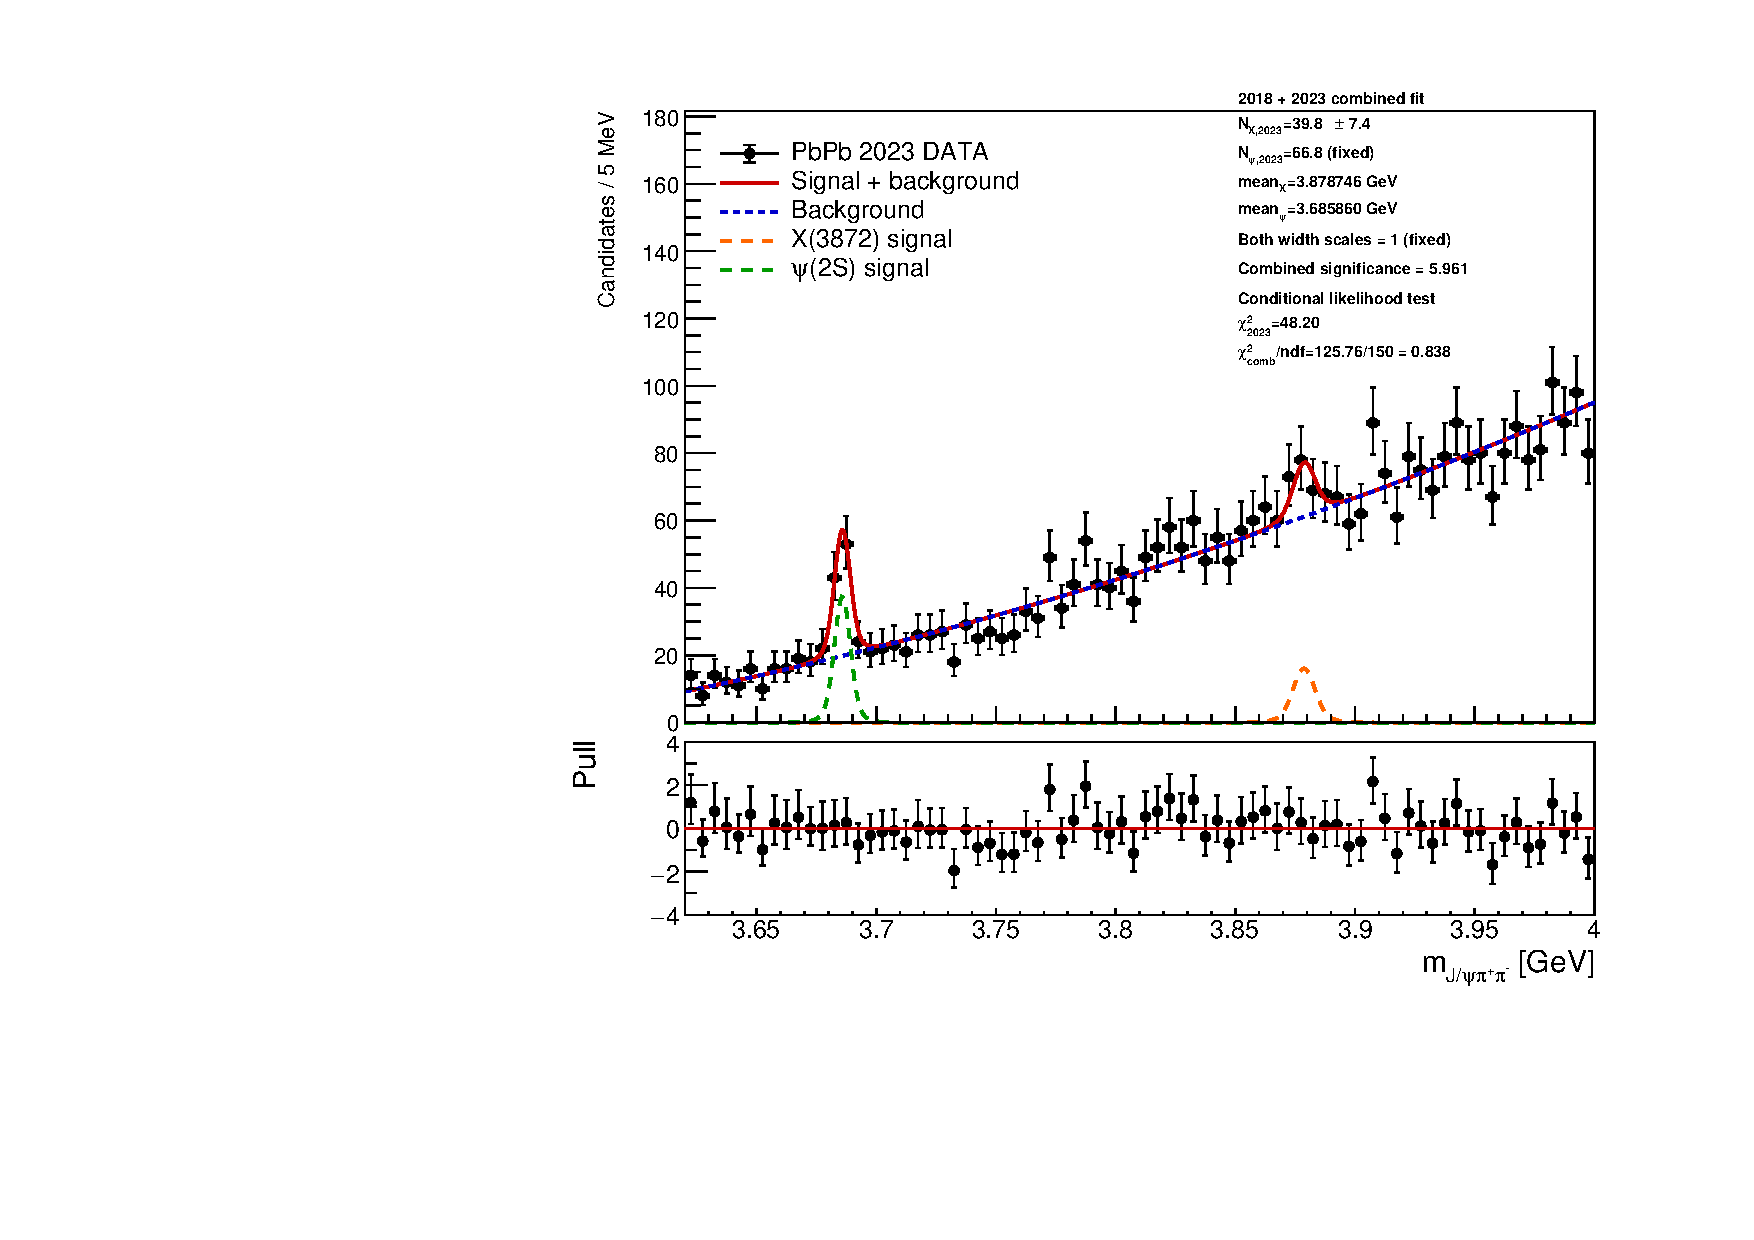
\includegraphics[width=\linewidth,height=0.58\textheight,keepaspectratio]{figures/20260930/3v12/pb23_conditional_fit.pdf}
\end{columns}\small
\textbf{Combined:} $N_X=130.38\pm24.21$; significance $=5.961\sigma$.\par
\textbf{Independent-year reference:} 2018: $5.400\sigma$; 2023: $2.460\sigma$.\par
\textbf{Combined:} $\chi^2/\mathrm{ndf}=0.838$.\par
\caution{MC double-Gaussian widths fixed; 2nd-order Chebyshev background.}

\end{frame}

